As pointed out in \cite{hobor:ramification}, na\"iave attempts to
verify graph-manipulating programms using the shape-only predicates
are unsound. An obvious solution---especially for verifying functional
correctness---is to involve a mathematical graph $\gamma$ in spatial
predicates as a parameter. Since the additional parameter is involved
in the specification, we needs a way to reason about it, so as to
deduce the specification. Thus we formalize a proof framework for
mathematical graphs and provide a bunch of useful theorems in graph
theory to ease the burden in verifying programs. In this section, we
will introduce the framework and show how we built them.

\subsection{Definitions of graph and other concepts}

The core of the graph theory framework are the definitions of graph,
graph-related structures and relations. In mathematics, a (directed)
graph is an ordered pair $(V, E)$ where $V$ is a set of vertices or
nodes and $E$ is a set of edges comprising a source node and a
destination node. In our framework, we defined a similar structure
with minor amendment: we attached ``validity'' property to each vertex
and edge while $V$ and $E$ serve as types instead of sets of vertices
and edges respectively. There are two reasons for the amendment. The
first is that in many proof assistants, it is much easier and natural
to declare types instead of sets. When using types, validity is an
effective way in controlling membership: most graphs do not contain
all instances of vertex type and edge type. The second reason is
expanding the scope of representation, not just normal graphs. For
example, in some cases, we need to describe the difference of two
graphs: $\gamma_1-\gamma_2$, which is not necessarily a graph because
it may contain dangling edges. The ``subtracted'' nodes are not really
removed but are ruled out from valid nodes because they are still
referred in edges part of the definition of $\gamma_1-\gamma_2$. So we
call this structure \textbf{PreGraph}, which means it may be
incomplete in comparison with a classical graph. In our framework, a
PreGraph $\gamma$ is a hextuple $(V, E, \Phi_V, \Phi_E, s, t)$ where
$\Phi_V$ and $\Phi_E$ are validity predicates for vertex type $V$ and
edge type $E$, $s$ and $t$ are functions which takes an edge as
argument and returns source/destination node of the edge. Many
concepts such as reachability, subgraph and structural equivalence are
defined based on PreGraph.

\paragraph{Path}
Once we have the definition of PreGraph, it is time to define another
infrastructure: path. Informally, a path is a list of nodes
concatenated with edges. Since an edge contains the information about
its source and destination nodes, there is no necessary to define path
as an interleaving list of nodes and edges. Then we have two obvious
choices for representation of a path: a list of nodes or a list of
edges.

Both choices have certain defects. If a path is defined as a list of
nodes, we can not distinguish different paths between two nodes in
case there are multiple edges between two nodes. If a path is defined
as a list of edges, then we can deal with multiple edges but we can
not represent an empty path for a certain node---we can not determine
which node an empty list of edges belongs to.

To avoid the defects above, we define the path as a ordered pair $(n,
l)$ where $n$ is a node and $l$ is a list of edges. A valid path
requires that $n$ is the source node of the first edge of $l$ and $l$
is well chained---the destination of an edge in $l$ is the same as the
source of the next edge. The list $l$ can be null to represent an
empty path for a particular node $n$.

Why we insist that a path---even an empty path---must have a leading
node? One reason is that with such a definition, we can give a
consistent definition for a very important concept: reachability.

\paragraph{Reachability}
Among various properties derived from PreGraph, the most important one
is the reachability. The definition of reachability is based on
path. The notation $\gamma \models L_{n_2}^{n_1}(P)$ means in PreGraph
$\gamma$, node $n_2$ is reachable from node $n_1$ along the path $L$
while every node in $L$ satisfies predicate $P$. This notation, along
with other derived ones, such as
\begin{equation*}
\begin{split}
\gamma\models n_1 \xrightarrow{P} n_2 &\triangleq \exists L, \gamma \models L_{n_2}^{n_1}(P),\\
\gamma\models n_1 \leadsto n_2 &\triangleq \exists L, \gamma \models L_{n_2}^{n_1}(True)
\end{split}
\end{equation*}
form the bedrock of nearly every nontrivial predicate about
graph. Either the relation of two states---before and after running an
algorithm---of a graph or the description of a graph with a particular
shape, reachability is inevitable. To some extent, it is quite natural
because most graph-related algorithms (DFS, BFS, Shortest Path,
Spanning Tree, etc) depend on a small operation: exploring neighbours
from one node. Thus when describing the effect of an algorithm,
reachability is indispensable. Some of those descriptions are
discussed in later sections.

\paragraph{Subgraph}
When we tie a mathematical graph $\gamma$ to a spatial graph predicate
$g(x, \gamma)$ (which will be explained later), $g$ ``owns'' only the
spatial representation of the portion of $\gamma$ that is reachable
from $x$; $\gamma$ may contain other nodes. When we reason about
$g(x, \gamma)$, it is a very natural requirement to describe the
reachable portion of $\gamma$ in pure part. We generalize this
description as two concepts: partial graph $\gamma \!\uparrow\! P$ and
subgraph $\gamma \!\downarrow\! P$ for arbitrary predicate $P$. To define
$\gamma \!\uparrow\! P$ and $\gamma \!\downarrow\! P$, for any $\gamma=(V,
E, \Phi_V, \Phi_E, s, t)$, we do not change $V$ and $E$ but change
$\Phi_V$ and $\Phi_E$ by adding proposition about satisfying $P$ for
nodes. It means valid nodes in $\gamma \!\uparrow\! P$ and
$\gamma \!\downarrow\! P$ must satisfy $P$. The only difference between
$\gamma \!\uparrow\! P$ and $\gamma \!\downarrow\! P$ is that in
$\gamma \!\uparrow\! P$ the edges with its source node satisfying $P$ is
valid, but in $\gamma \!\downarrow\! P$, valid edges means both its source
and destination nodes satisfy $P$. With the concepts of partial graph
and subgraph, we can express the reachable portion by instantiating
$P$ as reachable predicate.

\paragraph{Structural Equivalence}
Many graph-manipulating algorithms adopt divide and conquer
paradigm. Most of those algorithms contain certain invariants as parts
of their specifications. Usually it means certain portion of graph
before program execution is equivalent to the one after execution. To
describe this relation, we introduced ``structural equivalence'' in
our framework with the following definition:
\begin{equation*}
\begin{split}
\gamma_1 \cong\gamma_2 \triangleq & \forall v, \Phi_{V1}(v) \leftrightarrow \Phi_{V2}(v) \wedge \\
& \forall e, \Phi_{E1}(e) \leftrightarrow \Phi_{E2}(e) \wedge\\
& \forall e, \Phi_{E1}(e) \rightarrow \Phi_{E2}(e) \rightarrow \text{src}_{\gamma_1}(e)=\text{src}_{\gamma_2}(e) \wedge\\
& \forall e, \Phi_{E1}(e) \rightarrow \Phi_{E2}(e) \rightarrow \text{dst}_{\gamma_1}(e)=\text{dst}_{\gamma_2}(e)\\
\end{split}
\end{equation*}
Informally it means $\gamma_1$ and $\gamma_2$ has the same vertex set
and edge set. And any valid edge in both graphs is comprised by the
same source and destination nodes. This relation can be used with
subgraph and reachability to define many concrete relations in program
verification.

\subsection{Classification of various graphs}

PreGraph and its derived properties (reachability, subgraph, etc) are
inadequate for real program verifications. Admittedly many helpful
lemmas can be inferred directly from PreGraph. But when we dealing
with concrete graphs for various algorithms, there are many features
which a bare PreGraph can not inculde. For example, when we compute
some properties of a graph, we always hope the graph is finite
connected. In the recursive defnition of a graph data structure, a
node contains many pointers to point to its neighbors. The pointers
could be null to indicate that they do not point to any. Thus we need
a special node which represents null pointer. In some cases, we have
to specify a graph in which the outdegree of each nodes is 2. All
these additional properties are abstracted as different property
bundles. We defined \textbf{LocalFiniteGraph}, \textbf{MathGraph}
and \textbf{BiGraph} for the three requirements above,
respectively.

\begin{figure}[htbp]
\centering
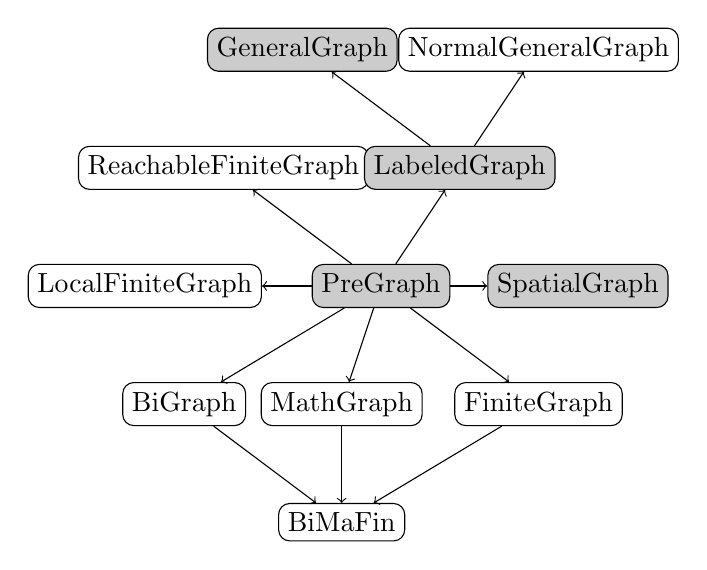
\begin{tikzpicture}%[->/.tip={Stealth}]
\tikzstyle{every node}=[shape=rectangle, rounded corners=4pt, draw]
\node[fill=gray!40] (GG) at (1, 6) {GeneralGraph};
\node (NGG) at (4, 6) {NormalGeneralGraph};
\node (RFG) at (0, 4.5) {ReachableFiniteGraph};
\node[fill=gray!40] (LG) at (3, 4.5) {LabeledGraph};
\node (LFG) at (-1, 3) {LocalFiniteGraph};
\node[fill=gray!40] (PG) at (2, 3) {PreGraph};
\node[fill=gray!40] (SG) at (4.5, 3) {SpatialGraph};
\node (BG) at (-0.5, 1.5) {BiGraph};
\node (MG) at (1.5, 1.5) {MathGraph};
\node (FG) at (4, 1.5) {FiniteGraph};
\node (BMF) at (1.5, 0) {BiMaFin};
\draw [->] (LG) to (NGG);
\draw [->] (LG) to (GG);
\draw [->] (PG) to (LG);
\draw [->] (PG) to (SG);
\draw [->] (PG) to (RFG);
\draw [->] (PG) to (LFG);
\draw [->] (PG) to (BG);
\draw [->] (PG) to (MG);
\draw [->] (PG) to (FG);
\draw [->] (BG) to (BMF);
\draw [->] (MG) to (BMF);
\draw [->] (FG) to (BMF);
\end{tikzpicture}
\caption{Various Kinds of Graphs}\label{fig:graphs}
\end{figure}

As shown in Figure \ref{fig:graphs}, there are several different
``Graph'' definitions in our framework. Some of them (with gray
background) are real mathematical objects, just like PreGraph. The
rest are just property bundles which are PreGraph with special
properties. They provide different views of graphs from a certain
perspective.

In our framework, there are four kinds of \emph{real}
graphs: \textbf{PreGraph}, \textbf{SpatialGraph}, \textbf{LabeledGraph}
and \textbf{GeneralGraph}. The definition of PreGraph is already
known. Based on PreGraph, each node and each edge in a LabeledGraph
has extra labels which can be seen as label functions of nodes and
edges. A GeneralGraph is a LabeledGraph with a customized sound
condition. A SpatialGraph is the graph directly stored in memory,
which contains connecting and user specified informations stored on
every vertex and/or every edge.

The rest in Figure \ref{fig:graphs} are all property bundles where
LocalFiniteGraph, MathGraph and BiGraph are already explained. A
FiniteGraph is a graph with finite number of vertices and edges. (So a
FiniteGraph is definitely a LocalFiniteGraph.) A BiMaFin is a graph
satisfying BiGraph, MathGraph and FiniteGraph simultaneously. A
ReachableFiniteGraph is a graph in which all reachable nodes of an
arbitrary node are finite. A NormalGeneralGraph is a special
GeneralGraph used for certain algorithms. Usually in the correctness
proofs of concrete algorithms, all graphs satisfy the definition of
BiMaFin, LocalFiniteGraph, ReachableFiniteGraph and etc. But for many
math theorems in graph theory, some properties (e.g. FiniteGraph,
BiGraph) are not necessary. These different properties for different
theorems make our framework more flexible and general.

\subsection{Computable Reachability}
We proved quite many property-bundle specific theorems. One typical
example of such theorems is the following one:
\newtheorem{mythm}{Theorem}
\begin{mythm}
For any graph $\gamma$ which is both MathGraph and LocalFiniteGraph
and any node $x$ in $\gamma$, if the number of nodes reachable from
node $x$ is finite, then we can find a set which exactly contains the
reachable nodes from $x$ in $\gamma$.
\end{mythm}
It sounds so trivial but the proof is totally non-trivial. The most
obvious way to prove it---filtering reachable nodes from all valid
nodes---is impossible: there is no decision procedure for reachability
to select reachable nodes because the current definition of graphs is
applicable for graphs containing infinite number of nodes (A
LocalFiniteGraph can still be infinite). In such a graph, one may need
to inspect infinite number of paths to judge whether a node is
reachable, which is a mission impossible.

Another intuitive way to construct the reachable list is using a
breadth-first searching algorithm to collect distinct nodes along the
edges from $x$, which is employed in the proof. But still, a na\"ive
implementation may not terminate. As mentioned in the premises of this
lemma, the number of reachable nodes has an upper bound. So the
actually working breadth-first searching function is constructed as
follows. It holds a set of nodes collected so far and a queue for
visited but unexpanded nodes. It keeps on expanding nodes from the
queue to add distinct nodes to result set and the processing queue,
until the processing queue is empty or the number of nodes collected
reaches the upper bound. It is worth mentioning that constructing this
function in Coq is hard. The direct implementation is rejected because
it violates the syntactic criteria for recursion in Coq. It has to be
defined in a sophisticated way: defining a well-founded relation and
proving that the definition of the function fulfills the relation.

After the establishing of the searching function, it is still hard to
prove that the result generated by the function is the reachable
list. There are two goals that needs to be proved: one is that all
nodes collected by this searching function is reachable from $x$ and
the other is all reachable nodes from $x$ is in the
collected list of the searching function. The former one is relatively
easier than the latter because for the latter case, there are two
completeness proofs corresponding to the two different termination
conditions. It is not known yet whether a proof by contradiction
exists or is simpler.

\subsection{Application of the framework}

Graph-manipulating programms may also deal with other structures, such
as dag (directed acyclic graph), tree or spanning tree. With the basic
defintions in our framework, new structures can be defined
easily. Acyclic graph is just a graph with an additional property:
forall any $x$ and $y$, if $x$ is reachable from $y$, then $y$ is not
reachable from $x$. Tree is similar. The additional property for tree
is that there is one and only one path from root to any reachable node
from root. Spanning tree is a tree with the same reachable vertex set
of the original graph.

But when dealing with formal proofs, there are some unexpected
facts. For example, our na\"ive definition of the
predicate \verb|spanning_tree| is not strong enough to complete the
inference. We express that graph $g_2$ is a spanning tree of graph
$g_1$ starting from root node $r$ as \verb|spanning_tree|
$g_1\,r\,g_2$. We conclude three relations as the predicate. First,
the unreachable parts from root $r$ in $g_1$ and $g_2$ are the
same. Secondly, the shape of $g_2$ must be a tree. Lastly, all nodes
reachable from $r$ in $g_1$ are still reachable from $r$ in $g_2$. The
second relation ensures that the result is a tree while the third one
ensures it is a spanning tree of $g_1$. At first glance, it is a very
complete definition. But the subsequent formal proof reveals that the
definition still lacks one condition: for any two nodes $a$ and $b$,
if $a$ is reachable from $r$ in $g_1$ and $b$ is not reachable from
$r$ in $g_1$, then in $g_2$, $b$ is not reachable from $a$. It is a
long-winded but necessary relation.
